\documentclass[12pt]{article}

% ---------- PREAMBLE ----------
\usepackage[utf8]{inputenc}
\usepackage[T1]{fontenc}
\usepackage{lipsum} % for dummy text, remove later

% Formatting
\usepackage{geometry}
\geometry{margin=1in}

% TOC + hyperlinks
\usepackage[colorlinks=true, linkcolor=blue, urlcolor=blue]{hyperref}
\usepackage{xcolor}
\usepackage[dvipsnames]{xcolor}
\usepackage{bookmark} % better PDF bookmarks

% Math
\usepackage{amsmath, amssymb}
\usepackage{cancel}

% Headers/footers
\usepackage{fancyhdr}
\pagestyle{fancy}
\fancyhf{} % clear all
\fancyfoot[C]{\thepage} % centered page number
\fancyhead[L]{ECE 6250 Fall 2025}
\fancyhead[R]{\leftmark} % week name in header (set via \markboth{}{})

% Images
\usepackage{graphicx}
\usepackage{float}
\graphicspath{{images/}}

% MATLAB code snippets
\usepackage{listings}

\lstset{
    language=Matlab,
    basicstyle=\ttfamily\small,
    keywordstyle=\color{blue},
    commentstyle=\color{green!50!black},
    stringstyle=\color{red},
    numbers=left,
    numberstyle=\tiny,
    stepnumber=1,
    numbersep=5pt,
    breaklines=true,
    showstringspaces=false,
}

% ---------- CUSTOM COUNTERS ----------

% Non-Numbered Subsection
\newcommand{\introsection}[1]{%
  \subsection*{#1}% print the subsection header
  \addcontentsline{toc}{subsection}{#1}% add to TOC
}

% Numbered subsections with auto-increment
\newcounter{lecture}[section] % reset at each week (section)
\renewcommand{\thelecture}{Lecture \arabic{lecture}}
\newcommand{\lecture}[1]{%
  \refstepcounter{lecture}%
  \subsection*{\thelecture: #1}%
  \addcontentsline{toc}{subsection}{\thelecture: #1}%
}

% Make equation numbering depend on lecture number e.g. (1.1), (1.2), and so on
\renewcommand{\theequation}{\arabic{lecture}.\arabic{equation}}
% Reset equations at the start of each lecture
\makeatletter
\@addtoreset{equation}{lecture}
\makeatother

% Same numbering logic as above but for figures instead of lectures 
\renewcommand{\thefigure}{\arabic{lecture}.\arabic{figure}}
\makeatletter
\@addtoreset{figure}{lecture}
\makeatother

% ---------- DOCUMENT ----------
\begin{document}

% Title Page
\begin{titlepage}
  \centering
  {\Huge ECE 6270 - Advanced DSP Notes \par}
  \vspace{1cm}
  {\Large Ben Rotker \par}
  \vfill
  {\large \today \par}
\end{titlepage}

% Table of Contents
\tableofcontents
\newpage

\section*{Introduction}
\addcontentsline{toc}{section}{Introduction}

\introsection{About}
The goal of this document is to provide detailed notes that supplement the lecture material and provide quick lookups for formulas and concepts. It was inspired by Shuvo Newaz's lecture notes for ECE 6271 - Adaptive Filtering. 


\introsection{Disclaimer}
I did my best to closely follow the lectures when creating these notes; however, they may not be 100\% perfect or error free. Please treat them as a supplement to the course and double-check anything you're unsure about using the official course material.

\introsection{Github Information}
These notes are open source and hosted on GitHub. 
You can view the latest version, make corrections, or suggest improvements at:\\
\url{https://github.com/rotkstar/ECE6250-Advanced-DSP-Notes} \\
If you'd like to contribute, please open an issue or submit a pull request with your correction.

\newpage
% Week 1 lectures
\section*{Week 1}
\addcontentsline{toc}{section}{Week 1}
\markboth{Week 1}{}

\lecture{Sampling pt 1}
\color{ForestGreen}
\large{\textbf{Shannon-Nyquist}}
\color{Black}\\
Sampling is simply converting a continuous signal into discrete samples. 
\begin{equation}
    x[n] = x_c(nT)
\end{equation}
Where T is the sampling period or interval. In this course, square brackets denote discrete signals and parentheses denote continuous signals. \\
Questions: \\
\textbf{1) Can we reconstruct $x_c(t)$ from $x[n]$?} \\
Short answer: sometimes. When $x_c(t)$ is band limited, that is, the frequencies are zero beyond a certain point, that is,
\begin{equation}
    X_c(j\Omega) = 0 \quad \forall \quad |\Omega| \ge \frac{\pi}{T}
\end{equation}
Where 
\begin{equation}
X_c(j\Omega) = \int_{-\infty}^{\infty}X_c(t)e^{-j\Omega t} \quad dt
\end{equation}
and 
\begin{equation*}
    e^{-j \Omega t} = cos(\Omega t) - jsin(\Omega t) 
\end{equation*}
We're really projecting our time signal onto a frequency basis. We get a representation of our original function in frequency (where $\Omega$ is the frequency in radians). 
When x is bandlimited, the frequency of x is zero above a certain point. Thus we can reconstruct $x_c(t)$ from $x[n]$ as long as the sampling rate is $\ge$ twice the highest frequency in $x_c(T)$. This is the Nyquist Criterion:
\begin{equation}
    \frac{2\pi}{T} > 2 \Omega_{max} 
\end{equation}
\\
\textbf{2) How exactly do we reconstruct the signal?} \\
Answer: We reconstruct using a sinc interpolator. 
\begin{equation}
    x_r(t) = \sum_{n=-\infty}^{\infty} x[n]\frac{sin(\pi(t-nT)/T)}{\pi(t-nT)/T} 
\end{equation}
\begin{equation}
    = \sum_{n=-\infty}^{\infty} x[n] \underbrace{g_T (t-nT)}_{\text{shifted sinc}}
\end{equation}
Issue: the sinc function dies out as $\frac{1}{T}$, meaning it never dies out until T reaches infinity. So we're adding an infinite number of functions with infinite supports.
\begin{figure}[H]
    \centering
    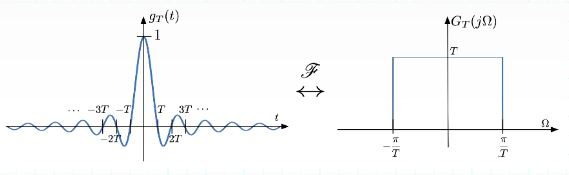
\includegraphics[width=0.75\linewidth]{6250-lecture01-img1.JPG}
    \caption{Sinc Function}
    \label{fig:placeholder}
\end{figure} 
\noindent The Fourier transform of the Sinc function is a rectangular box. We're basically taking our samples and filtering with an ideal LPF to ensure that we get our bandlimited signal back when we reconstruct it. \\
\begin{figure}[H]
    \centering
    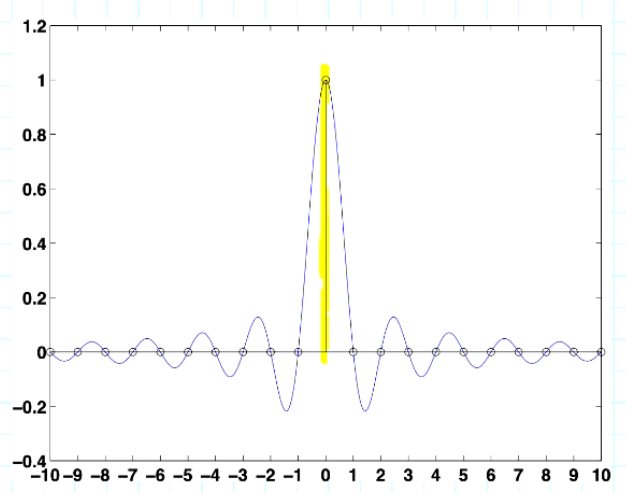
\includegraphics[width=0.5\linewidth]{6250-lecture01-im2.png}
    \caption{Unit Sample Reconstruction}
    \label{fig:placeholder}
\end{figure}
\noindent \textit{Figure 1.2} Shows the continuous signal reconstructed from the discrete unit sample using sinc interpolation. The sinc perfectly passes through zero at all the points equal to zero in the original unit sample (which is all the points except n=0). If we were to resample this continous signal once again, we would get the unit sample at n=0.\\
\noindent When we have multiple samples in our discrete signal and then reconstruct the continuous signal with sinc interpolation, 
\begin{figure}[H]
    \centering
    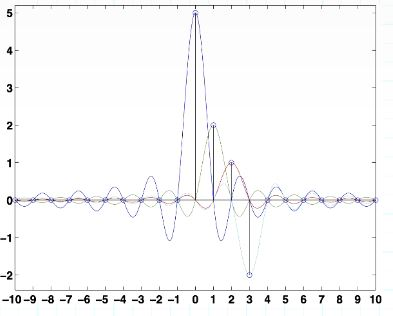
\includegraphics[width=0.5\linewidth]{ece6250-lecture01-img3.JPG}
    \caption{Multiple Samples Reconstruction}
    \label{fig:placeholder}
\end{figure}
\noindent We sum the colored sinc functions (one for each unit sample) to get our reconstructed continous signal. This may seem strange at first because we get little bumps added in like at n = -2.5. Intuituively, it would make more sense to just interpolate between each one of the unit samples; however, this version of the signal is bandlimited. While this sinc interpolation method isn't ideal for something like an image, it is best for a bandlimited signal, which is what we're typically concerned with. \\
\color{ForestGreen}
\large{\textbf{Fundamental Theorem of DSP}}
\color{Black}\\
\noindent If $x_c(t)$ is bandlimited to B ($X_c(j \Omega) = 0$ for $|\Omega| > B$), then it can be perfectly reconstructed from samples spaced T \leq $\pi /B$ apart. 
\begin{equation}
    x_c(t) = \sum_{n=-\infty}^{\infty}x[n]g_T(t-nT)
\end{equation}
Where 
\begin{equation*}
    x[n] = x_c(nT) \qquad g_T(t) = \frac{sin(\pi t/T)}{\pi t/T}
\end{equation*}

\newpage
\lecture{Sampling pt 2}
\color{ForestGreen}
\large{\textbf{Frequency Domain Interpretation}}
\color{Black}\\
So far, we have said that samples are simply the continuous-time signal evaluated at periodic points, separated by a distance T. We need to discuss some intermediate steps here. \\
\textbf{Step 1:} Multiply continuous-time signal by a delta function. \\ 
There are two types of delta functions: \\ \\
a) The Kroenecker delta (discrete time) is 0 everywhere except n=0, 
where it is equal to one.\\ 
b) The Dirac delta function (continuous time) integrates to 1. 
\begin{figure}[H]
    \centering
    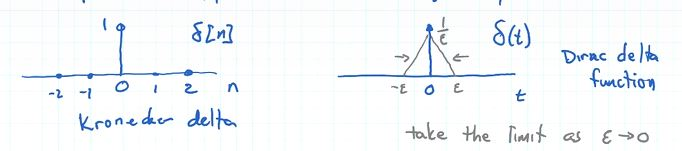
\includegraphics[width=0.75\linewidth]{ece6250-lecture02-img1.JPG}
    \caption{Kronecker and Dirac Delta Functions}
    \label{fig:placeholder}
\end{figure}
The Dirac delta function has some interesting properties: \\ \\
a) $\int_{-\infty}^{\infty} \delta (t) = 1$ \\
b) $\delta (t) = 0 $ if $t \neq 0$ \\
c) $x(t) \delta(t-t_0) = x(t_0) \delta(t-t_0)$ \\ \\
We define the DTFT as: 
\begin{equation}
    X(e^{j\omega})  \overset{\Delta}{=} \sum_{n=-\infty}^{\infty}x[n]e^{-j \omega n}
\end{equation}
\begin{equation*}
    X(e^{j\omega}) = \sum_{n=-\infty}^{\infty}x_c(nT)e^{-j \omega n}
\end{equation*}
We can express $x_c$ in terms of its Fourier transform. \\
\begin{equation*}
    = \sum_{n=-\infty}^{\infty}\left(\frac{1}{2\pi} \int_{-\infty}^{\infty} X_c(j \Omega) e^{-j \Omega nT} d\Omega\right)e^{-j \omega n}
\end{equation*}
Rearranging terms, we get\\
\begin{equation*}
    = \frac{1}{2 \pi} \int_{-\infty}^{\infty} X_c(j \Omega) \left(\sum_{n=-\infty}^{\infty} e^{j n(\Omega T - \omega)}\right) d\Omega
\end{equation*}
Unfortunately, we hit a roadblock here in that we have an infinite sum. \\
Luckily, we can leverage the Poisson summation formula: \\
\begin{equation}
    \sum_{n=-\infty}^{\infty} e^{jn\omega} = 2\pi \sum_{k=-\infty}^{\infty} \delta(\omega-2 \pi k)
\end{equation}
Plugging this in, we get
\begin{equation*}
    = \cancelto{1}{\frac{2 \pi}{2 \pi}} \int_{-\infty}^{\infty} X_c(j \Omega) \left( \sum_{k=-\infty}^{\infty} \delta(\Omega T - \omega - 2 \pi k)\right) d\Omega
\end{equation*}
Switching the order of summation and integration: \\
\begin{equation*}
     = \sum_{k=-\infty}^{\infty} \int_{\Omega}^{} X_c(j \Omega) \delta(\Omega T - \omega - 2 \pi k) d\Omega
\end{equation*}
We can swap $\Omega = (\omega + 2 \pi k)/T$ because this causes the argument of the delta function to be zero, which is the only point where the delta function is nonzero. \\
\begin{equation}
    = \frac{1}{T} \sum_{k=-\infty}^{\infty} X_c\left(j \frac{\omega + 2\pi k}{T}\right)
\end{equation}
We're taking our original continuous time signal spectrum and summing infinitely many copies of it together, each one spaced by $2 \pi k$. \\
The $1/T$ in the argument of $X_c$ dilates the spectrum (stretches it out). \\

\newpage
\lecture{Sampling pt 3}
\color{ForestGreen}
\large{\textbf{Frequency Domain Interpretation (continued)}}
\color{Black}\\
B is the continuous-time frequency in radians. We get aliasing if $B > \pi/T$, i.e. $f_{max} < f_s/2$. In words, this is corruption of the spectrum by one of the copies of the period.\\
Last lecture, we discussed reconstructing signals using infinite sums. Regarding computational complexity, infinite sums are obviously not ideal, so we need an alternative. 
\begin{equation}
    x_r(t) = \sum_{n=-\infty}^{\infty} x[n] g_T (t-nT)
\end{equation}
\begin{equation}
    \Rightarrow X_r(j \Omega) = \sum_{n} x[n] G_T (j \Omega) e^{-j \Omega n T}
\end{equation}
The Fourier transform is not a function of n, so it can come out front. 
\begin{equation*}
    = G_T(j\Omega) \sum_n x[n] e^{-j \Omega n T}
\end{equation*}
If $ \omega = \Omega T$, then this is the DTFT spectrum of x[n]. $\Omega T$ dilates the spectrum.
\begin{equation}ss
    X_r(j \Omega) = G_T(j \Omega) X(e^{j \Omega T})
\end{equation}
The figures below outline the process of creating a continuous-time signal from discrete samples, viewed through the frequency domain. 
\begin{figure}[H]
    \centering
    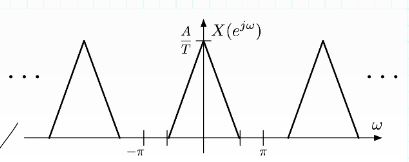
\includegraphics[width=0.75\linewidth]{ece6250-lecture03-img1.JPG}
    \caption{DTFT Spectrum}
    \label{fig:placeholder}
\end{figure}
\textit{Figure 3.1} shows the DTFT spectrum of a sampled signal. 
\begin{figure}[H]
    \centering
    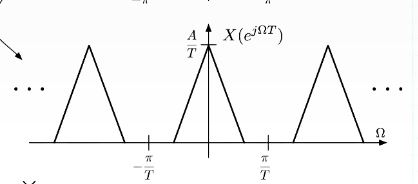
\includegraphics[width=0.75\linewidth]{ece6250-lecture03-img2.JPG}
    \caption{Spectrum of x(nT)}
    \label{fig:placeholder}
\end{figure}
\noindent The first step in converting this signal to continuous-time is by turning the scaled and shifted Kronecker delta functions (1 per sample) into scaled and shifted Dirac delta functions (1 per sample).
\begin{figure}[H]
    \centering
    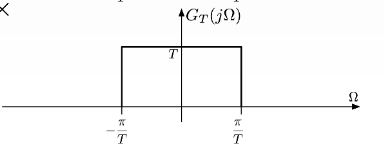
\includegraphics[width=0.75\linewidth]{ece6250-lecture03-img3.JPG}
    \caption{Interpolation Function Spectrum}
    \label{fig:placeholder}
\end{figure}
\noindent Next, we filter these Dirac delta functions using our filter, i.e. we convolve them with our $g_T$ function. 
\begin{figure}[H]
    \centering
    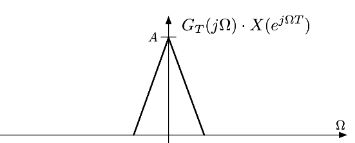
\includegraphics[width=0.75\linewidth]{ece6250-lecture03-img4.JPG}
    \caption{Continuous-Time Signal Spectrum}
    \label{fig:placeholder}
\end{figure}
\noindent This gives us our continuous-time signal, the spectrum of which is shown in \textit{Figure 3.4}. \\
As we have stated several times, the sinc function is infinite in length. There are a couple approximate reconstruction techniques we can use instead. \\
The first is "sample and hold". Draw a horizontal line at the height of the current sample, from the current sample to the next. This creates a piecewise continuous function, and yields a $G_T(j \Omega) $ that is a sinc in the frequency domain. This is not ideal - the frequency content of the signal becomes distorted because the passband isn't flat, and because we've added in frequency content from neighboring replications. \\
A better alternative is linear interpolation. The frequency domain transform of a linear interpolator is a triangle function. We're still distorting the spectrum, but less so than with sample and hold interpolation. \\
Whatever we choose as our interpolator, we can think of it as an impulse response of some filter in the frequency domain. One thing we can do to make it work better is ensure that we're sufficiently sampled. \\

\newpage
% Week 2 lectures
\section*{Week 2}
\addcontentsline{toc}{section}{Week 2}
\markboth{Week 2}{}

\lecture{Basis Expansions}

Last time we found that we could sample a continuous time signal into a list of numbers $x[n]$, and perfectly reconstruct that continuous time signal, at least theoretically. This is really remarkable because we can map a sequence of infinite points to a countable number of points indexed by n, $x[n]$. But this only works because $x(t)$ is band-limited. So with that extra constraint, we know that we can take some continuous signal and we can turn it into a list of numbers that we can then analyze and operate on.

\begin{figure}[H]
    \centering
    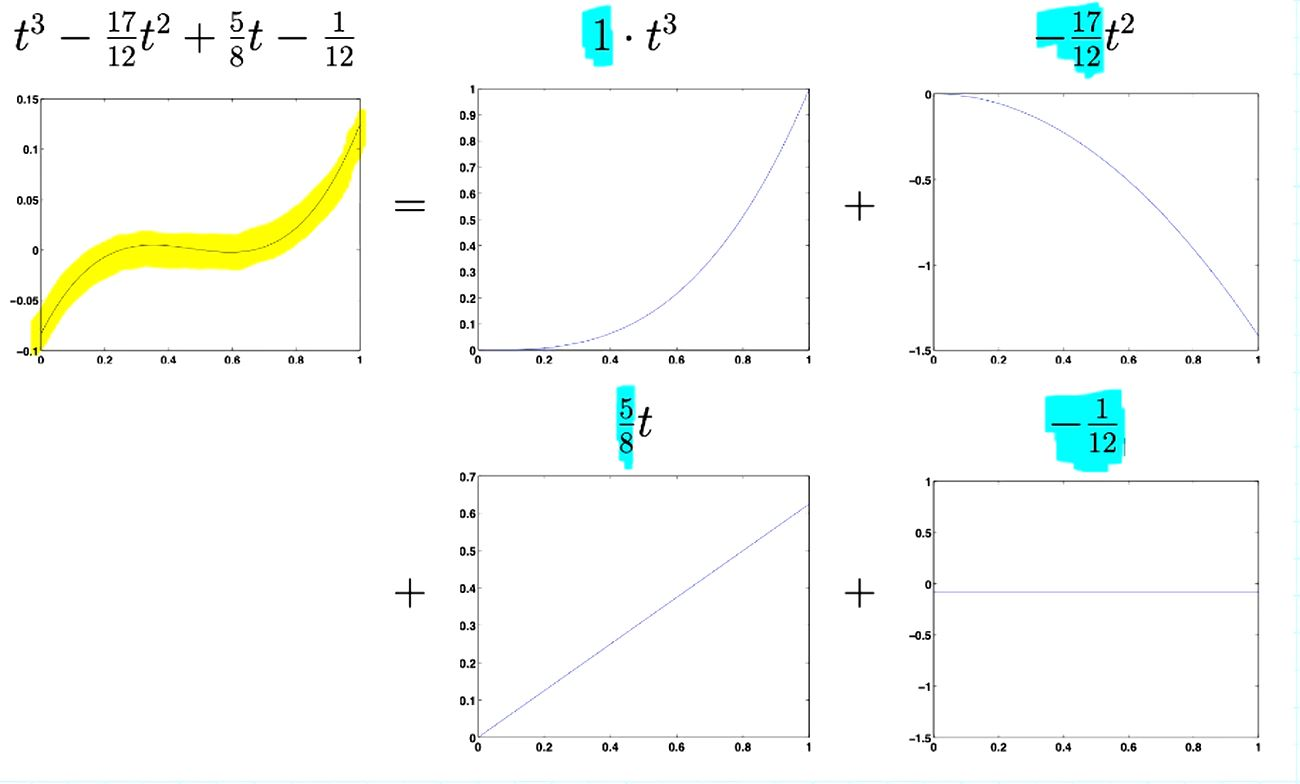
\includegraphics[width=0.75\linewidth]{6250-L4-IMG1.JPG}
\end{figure}

There are other ways that we can take a continuous signal and come up with a list of numbers. For example, in the leftmost block above, we have a continuous signal on the interval $[0,1]$ represented by a polynomial. This polynomial signal is really just a list of four numbers, which are the coefficients for each of the powers of t. Although we're only using up to the power of three in this example, we could go up to infinite order. If we take our coefficients to be the k derivatives evaluated at zero all over k factorial, we come up with the Taylor series:

\begin{equation}
    x(t) = \sum_{k=0}^{\infty} \alpha_k t^k \quad \text{if} \quad  \alpha_k = \frac{x^{(k)}(0)}{k!}
\end{equation}

Alternatively, we could use Lagrange Polynomials or B-Splines:

\begin{equation}
    x(t) = \sum_{k=0}^{M} \alpha_t P_k(t) 
\end{equation}

We cannot take an arbitrary continuous signal and turn it into a list of numbers until we put some constraints on it, because we initially have an uncountable, infinite number of degrees of freedom. In the polynomial example, the constraint is a differentiable signal that is limited to the interval [0,1].

\[
\boxed{\parbox{0.9\textwidth}{\centering
Ultimate goal: Represent continuous signals in a discrete way to enable the use of linear algebra for processing
}}
\]

\lecture{Vector Spaces}
$\textbf{S}$ : a vector space composed of a set of elements, called vectors, and members of a field $\mathbb{F}$ called scalars. 
Rules for addition and multiplication by scalars:
\begin{itemize}
    \item Vector addition (+) combines two vectors into a third
    \item Scalar multiplication combines a scalar and vector to produce another vector 
\end{itemize}
Addition: The '+' operation obeys four rules for all $\textbf{x}, \textbf{y} \in \textbf{S}$
\begin{enumerate}
    \item $\textbf{x} + \textbf{y} = \textbf{y} + \textbf{x}$ (commutative)
    \item $\textbf{x} + (\textbf{y} + \textbf{z}) = (\textbf{x} + \textbf{y})+\textbf{z}$ (associative)
    \item There is a unique zero vector, \textbf{0}, s.t. $ x+\textbf{0} = \textbf{x} \quad \forall \textbf{x} \in \textbf{S}$
    \item For each $\textbf{x} \in \textbf{S}$, there is a unique vector called $-\textbf{x}$ such that $\textbf{x} + (-\textbf{x}) = 0$
\end{enumerate}
Scalar multiplication: For $a, b \in \mathbb{F}$ and $\textbf{x}, \textbf{y} \in \textbf{S}$, scalar multiplication must obey
\begin{enumerate}
    \item $a(\textbf{x}+\textbf{y}) = a\textbf{x} + a\textbf{y}$ and $(a+b)\textbf{x} = a\textbf{x} + b\textbf{x}$ (distributive)
    \item $(ab)x = a(bx)$ (associative)
    \item for the multiplicative identity in $\mathbb{F}$, 1, we have $1\textbf{x} = \textbf{x} \quad \forall \textbf{x} \in \textbf{S}$
    \item for the additive identity in $\mathbb{F}$, 0, we have $0 \textbf{x} = \textbf{0}$
\end{enumerate}
$\textbf{S}$ is closed under vector addition and scalar multiplication. 
\begin{equation}
    \boxed{\textbf{x}, \textbf{y} \in \textbf{S} \Rightarrow a\textbf{x} + b \textbf{y} \in \textbf{S} \quad \forall a,b \in \mathbb{F}}
\end{equation}
This means that using the above operations, we will always get something back that is within our vector space.
Some examples of vector spaces:
\begin{enumerate}
    \item $\mathbb{R}^N$
    \begin{equation*}   
        \begin{bmatrix}
            x_1 \\
            \vdots \\
            x_N
        \end{bmatrix}
        \quad \text{where $x_i$ are real}
    \end{equation*}
    \text{with scalars as real numbers,using standard mult. and addition}
    \item $\mathbb{C}^N$, same as above but with complex $x_i$ and scalars. 
    \item Galois Field $GF(2)^N$, the scalar field is ${0, 1}$, so vectors are lists of N bits.
    \text{Addition is modulo 2.}\\
    $0 + 0 = 0$\\
    $0 + 1 = 1 + 0 = 1$\\
    $1 + 1 = 0$\\
    \begin{equation*} 
        \textbf{x} = 
        \begin{bmatrix}
            b_1 \\
            \vdots \\
            b_N
        \end{bmatrix}
        \Rightarrow_{\text{Example}}
        \begin{bmatrix}
            1 \\
            1 \\
            0 \\
            1
        \end{bmatrix}
        +
        \begin{bmatrix}
            1 \\
            0 \\
            0 \\
            0
        \end{bmatrix}
        =
        \begin{bmatrix}
            0 \\
            1 \\
            0 \\
            1
        \end{bmatrix}
    \end{equation*}
    \item Bounded, continuous functions $f(t)$ on the interval $[a,b]$ that are real-valued. \\
    \text{\quad Vector addition $\Rightarrow$ pointwise addition of functions} \\
    \text{\quad Scalar mult. $\Rightarrow$ multiplying by $a \in \mathbb{R}$ pointwise} \\
\end{enumerate}
Example of \textbf{not} a vector space:
bounded, continuous functions $f(t)$ on $[a,b]$ such that $|f(t)|<2$. (Not closed)

\lecture{Linear Subspaces}
A (non-empty) subset $\textbf{T}$ of $\textbf{S}$ is called a linear subspace of $\textbf{S}$ if 
\begin{equation}
    \forall a,b \in \mathbb{F} ,\quad  \textbf{x}, \textbf{y} \in \textbf{T} \Rightarrow a\textbf{x} + b\textbf{y} \in \textbf{T}
\end{equation}
This implies $\textbf{0} \in \textbf{T}$. 
$\textbf{T}$ is also a vector space by itself. 

\newpage
\lecture{Linear Combinations and Spans}
\color{ForestGreen}
\large{\textbf{Linear Combinations}}
\color{Black}\\
Suppose we have some linear combination of vectors
\begin{equation*}
    a_1 \mathbf{v_1} + a_2 \mathbf{v_2} + \cdots + a_m \mathbf{v_m} \quad \text{for some }\quad a_1,\cdots,a_m \in \mathbb{F}
\end{equation*}
The span of a set of vectors in \textbf{S} is the set of all vectors that are linear combinations of that set. We write it as
\begin{equation*}
    \text{Span}(\{\mathbf{v_1}, \mathbf{v_2}, ..., \mathbf{v_m}\})
\end{equation*}
Suppose
\begin{equation*}
    \mathbf{v_1} = 
    \begin{bmatrix}
            1 \\
            1 \\
            0
    \end{bmatrix}, 
    \mathbf{v_2} = 
    \begin{bmatrix}
            0 \\
            1 \\
            0
    \end{bmatrix}
    \quad \mathbf{S} \in \mathbb{R}^3, \quad \mathbb{F} = \mathbb{R}
\end{equation*}
All linear combinations of $\mathbf{v_1} \text{ and } \mathbf{v_2}$ can be written as 
\begin{equation*}
    a
    \begin{bmatrix}
            1 \\
            1 \\
            0
    \end{bmatrix}
    + b
    \begin{bmatrix}
            0 \\
            1 \\
            0
    \end{bmatrix}
    = 
    \begin{bmatrix}
            x_1 \\
            x_2 \\
            0
    \end{bmatrix}
    \text{for any } \quad x_1, x_2 \in \mathbb{R}
\end{equation*}
\color{ForestGreen}
\large{\textbf{Linear Dependence}}
\color{Black}\\
A set of vectors $\{\mathbf{v_j}\}_{j=1}^N$ is linearly dependent if $\sum_{n=1}^N a_n\mathbf{v_n}=0$ for some set $a_1,...,a_n$ (where not all $a_n$'s are zero) \\
\newline
\color{ForestGreen}
\large{\textbf{Linear Independence}}
\color{Black}\\
$\sum_{n=1}^N a_n\mathbf{v_n}=0$ only for $a_n=0 \quad \forall n$ \\
\newline
\underline{Example 7.1} \\
\begin{equation*}
    \mathbf{S} = \mathbb{R}^3, \quad \mathbf{v_1} =
    \begin{bmatrix}
            2 \\
            1 \\
            0
    \end{bmatrix}
    \quad \mathbf{v_2} =
    \begin{bmatrix}
            1 \\
            1 \\
            0
    \end{bmatrix}
    \quad \mathbf{v_3} =
    \begin{bmatrix}
            1 \\
            2 \\
            0
    \end{bmatrix}
\end{equation*}
Find $a_1, a_2, a_3 \quad \text{such that} \quad a_1\mathbf{v_1} + a_2\mathbf{v_2} + a_3\mathbf{v_3} = 0$ \\
Note, any two of these are linearly independent. \\
\begin{equation*}
    \text{span}(\{\mathbf{v_1}, \mathbf{v_2}\}) = \text{span}(\{\mathbf{v_2}, \mathbf{v_3}\}) = \text{span}(\{\mathbf{v_1}, \mathbf{v_3}\})     
\end{equation*}
\underline{Example 7.2} \\
Let \textbf{S} be the set of continuous signals on $[0,1]$
\begin{equation*}
    \mathbf{S} = \mathbf{C}([0,1]) \quad \mathbf{v_1} = cos(2\pi t) \quad \mathbf{v_2} = sin(2\pi t) \quad \mathbf{v_3} = 2cos(2\pi t + \frac{\pi}{3}) 
\end{equation*}
Can we find a set $a_1, a_2, a_3 \neq 0$ such that the linear combination goes to zero? (i.e. are they linearly dependent)?\\
\newline
Suppose we have some set $ \{\mathbf{v_1},\mathbf{v_2}, ..., \mathbf{v_n}\}$ are dependent. Then
\begin{equation}
    \sum_n a_n \mathbf{v_n} = 0 \Rightarrow \mathbf{v_k} = \frac{1}{a_k} \sum_{n \neq k} a_n \mathbf{v_n} \quad \text{for} \quad  a_k \neq 0
\end{equation}
at least one vector may be removed without changing the span. We can repeat until we have a linearly independent set. \\
\newline
\color{ForestGreen}
\large{\textbf{Basis}}
\color{Black}\\
A \underline{basis} of a finite-dimensional vector space \textbf{S} is a set of vectors \textbf{B} such that
\begin{enumerate}
    \item span(\textbf{B}) = \textbf{S}
    \item \textbf{B} is linearly independent 
\end{enumerate}
The second condition ensures bases of \textbf{S} will have the same number of elements. \\
The \underline{dimension} of \textbf{S} is the number of elements required in a basis for \textbf{S}. \\
\underline{Example 7.3} \\
\begin{equation*}
    \mathbf{S} = \{\text{polynomials of degree at most p}\}
\end{equation*}
A basis for \textbf{S} is $\mathbf{B} = \{1, t, t^2,...,t^p\}$. \\
The dimension of \textbf{S} is $p+1$. \\

\newpage
\lecture{Norms and Inner Products}
\color{ForestGreen}
\large{\textbf{Norms}}
\color{Black}\\
A \underline{norm} $||\cdot||$ on a vector space \textbf{S} is a mapping
\begin{equation*}
    ||\cdot|| : \mathbf{S} \rightarrow \mathbb{R}
\end{equation*}
with the following properties for all $\mathbf{x}, \mathbf{y} \in \mathbf{S}$
\begin{enumerate}
    \item $||\mathbf{x}|| \geq 0 $ \quad and \quad $||\mathbf{x}|| = 0 \iff \mathbf{x} = \mathbf{0}$
    \item $||\mathbf{x + y}|| \leq ||\mathbf{x}|| + ||\mathbf{y}||$ \qquad (triangle inequality)
    \item $||a\mathbf{x}|| = |a| \cdot ||\mathbf{x}||$ \quad for any scalar a (homogeneity)
\end{enumerate}
Other definitions 
\begin{itemize}
    \item The \underline{length} of $\mathbf{x} \in \mathbf{S} $ is simply $||\mathbf{x}||$
    \item The \underline{distance} between $\mathbf{x}$ and $\mathbf{y}$ is $||\mathbf{x}-\mathbf{y}||$
    \item A linear vector space equipped with a norm is called a \underline{normed vector space}
\end{itemize}
\underline{Examples} \\
\begin{equation*}
   \mathbf{S} = \mathbb{R}^N \quad ||\mathbf{x}||_2 = (\sum_{n=1}^N |\mathbf{x}_n|^2)^{1/2} \qquad \text{(Euclidean or $\ell_2$-norm)}
\end{equation*}
\begin{figure}[H]
    \centering
    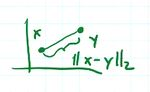
\includegraphics[width=0.5\linewidth]{6250-L08-IMG1.JPG}
\end{figure}
\begin{equation*}
    \mathbf{S} = \mathbb{R}^N \quad ||\mathbf{x}||_1 = \sum_{n=1}^N |\mathbf{x}_n| \qquad \text{(Manhattan norm)}
\end{equation*}
\begin{figure}[H]
    \centering
    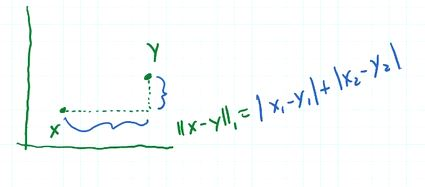
\includegraphics[width=0.5\linewidth]{6250-L08-IMG2.JPG}
\end{figure}
\begin{equation*}
    \mathbf{S} = \mathbb{R}^N \quad ||\mathbf{x}||_p = (\sum_{n=1}^N |\mathbf{x}_n|^p)^{1/p} \text{ for some } 1\leq p \leq \infty \qquad (\ell_p \text{ norm)}
\end{equation*}
\begin{equation*}
    \mathbf{S} = \mathbb{R}^N \quad ||\mathbf{x}||_{\infty} = \max\limits_{1,\dots,N} |\mathbf{x}_n| \qquad (\ell_{\infty} \text{ norm)}
\end{equation*}
\begin{figure}[H]
    \centering
    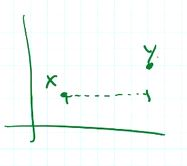
\includegraphics[width=0.5\linewidth]{6250-L08-IMG3.JPG}
\end{figure}
We can plot the unit ball of each norm as follows:
\begin{figure}[H]
    \centering
    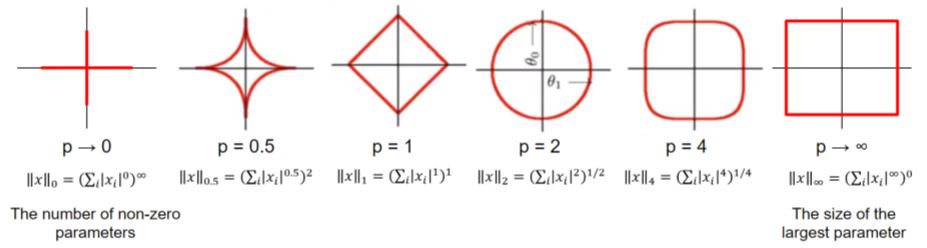
\includegraphics[width=1\linewidth]{6250-L08-IMG4.png}
\end{figure}
What if p=0? $\ell_0$ is \underline{not a norm}, it counts the number of nonzero elements. \\
\begin{equation*}
    \text{Ex. let }  
    \mathbf{x} = 
    \begin{bmatrix}
            3 \\
            2 \\
            0 \\
            0
    \end{bmatrix} 
    \text{ and } a=2. \quad ||a\mathbf{x}||_0 = 2 \neq |a|\cdot||\mathbf{x}||_0 = 2\cdot 2 = 4
\end{equation*}
\color{ForestGreen}
\large{\textbf{Inner Products}}
\color{Black}\\
An \underline{inner product} on a real or complex-valued vector space \textbf{S} is a mapping
\begin{equation*}
    \langle \cdot,\cdot \rangle : \mathbf{S} \times \mathbf{S} \rightarrow \mathbb{C}
\end{equation*}
That obeys 
\begin{enumerate}
    \item  $\langle \mathbf{x}, \mathbf{y} \rangle = \overline{\langle \mathbf{y}, \mathbf{x} \rangle} $ (Conjugate symmetry)
    \item $\langle a\mathbf{x} + b\mathbf{y},\mathbf{z} \rangle = a\langle \mathbf{x}, \mathbf{z} \rangle + b \langle \mathbf{y}, \mathbf{z} \rangle$ for any $a, b \in \mathbb{C}$ (Linearity)
    \item $\langle \mathbf{x}, \mathbf{x} \rangle \geq 0 $ and $\langle \mathbf{x}, \mathbf{x} \rangle = 0 \iff \mathbf{x} = \mathbf{0}$ (Positive definiteness)
\end{enumerate}
\underline{Common examples} 
\begin{itemize}
    \item $\mathbf{S} = \mathbb{R}^N \quad \langle \mathbf{x}, \mathbf{y} \rangle = \sum_{n=1}^N x_n y_n = \mathbf{y}^T \mathbf{x}$ \\ (All vectors in this class are column vectors unless otherwise noted)
    \item $\mathbf{S} = \mathbb{C}^N \quad \langle \mathbf{x}, \mathbf{y} \rangle = \sum_{n=1}^N x_n \overline{y_n} = \mathbf{y}^H \mathbf{x}$
    \item $\mathbf{S} = L_2[a,b] \quad \langle \mathbf{x}, \mathbf{y} \rangle = \int_a^b x(t)\overline{y(t)} dt$
\end{itemize}
\underline{Other (less common) examples} 
\begin{itemize}
    \item \textbf{S} = Gaussian RVs with zero-mean and finite variance \\
    \begin{equation*}
        \langle \mathbf{x}, \mathbf{y} \rangle = E[\mathbf{x}\mathbf{y}]
    \end{equation*}
    \item \textbf{S} = Differentiable, real-valued continuous signals on $\mathbb{R}$ \\
    \begin{equation*}
        \langle \mathbf{x}, \mathbf{y} \rangle = \int x(t)y(t) dt + \int x'(t) y'(t) dt    
    \end{equation*}
\end{itemize}
\underline{Induced norms}
A valid inner product induces a valid norm as 
\begin{equation*}
    ||\mathbf{x}|| = \sqrt{\langle \mathbf{x}, \mathbf{x} \rangle} 
\end{equation*}
Induced norms are norms (they obey all the properties we introduced previously). They also have additional properties. 
\begin{enumerate}
    \item Cauchy-Schwarz Inequality
    \begin{equation*}
        |\langle \mathbf{x}, \mathbf{y} \rangle| \leq ||\mathbf{x}||\cdot||\mathbf{y}||
    \end{equation*}
    Equality is only achieved when \textbf{x} and \textbf{y} are \underline{colinear}, meaning \\ $(\forall a \in \mathbb{C}, a \neq 0,$ such that $\mathbf{y} = a\mathbf{x})$
    \item Pythagorean Theorem 
    \begin{equation*}
        \langle \mathbf{x}, \mathbf{y} \rangle = 0 \Rightarrow ||\mathbf{x} + \mathbf{y}||^2 = ||\mathbf{x}||^2 + ||\mathbf{y}||^2 
    \end{equation*}
    Side note:
    \begin{equation*}
         \langle \mathbf{x+y}, \mathbf{x+y} \rangle =   \langle \mathbf{x}, \mathbf{x} \rangle +  \langle \mathbf{y}, \mathbf{y} \rangle
    \end{equation*}
    And we can also prove that 
    \begin{equation*}
         ||\mathbf{x} - \mathbf{y}||^2 = ||\mathbf{x}||^2 + ||\mathbf{y}||^2 
    \end{equation*}
    \item Parallelogram Law 
    \begin{equation*}
        ||\mathbf{x} + \mathbf{y}||^2 + ||\mathbf{x} - \mathbf{y}||^2  = 2||\mathbf{x}||^2 + 2||\mathbf{y}||^2 
    \end{equation*}
    \item Polarization Identity
    \begin{equation*}
        \operatorname{Re}\{\langle \mathbf{x}, \mathbf{y} \rangle \} = \frac{||\mathbf{x} + \mathbf{y}||^2 + ||\mathbf{x} - \mathbf{y}||^2}{4}
    \end{equation*}
\end{enumerate}
Aside: The angle between two vectors 
\begin{equation*}
    |\langle \mathbf{x}, \mathbf{y} \rangle| = ||\mathbf{x}||\cdot||\mathbf{y}|| \: cos(\Theta)
\end{equation*}
We can define the \underline{angle between two vectors} \textbf{x} and \textbf{y} in any inner product space as 
\begin{equation*}
    cos(\Theta) = \frac{\langle \mathbf{x}, \mathbf{y} \rangle}{||\mathbf{x}||\cdot||\mathbf{y}|| } \text{ if } \langle \cdot,\cdot \rangle \text{ induces } ||\cdot||
\end{equation*}
\newline
We can go even further and define \underline{orthogonality} : Vectors \textbf{x} and \textbf{y} in an inner product space are orthogonal to one another if $\langle \mathbf{x},\mathbf{y} \rangle=0$ \\
\color{ForestGreen}
\large{\textbf{Bonus: Plotting a Unit Ball}}
\color{Black}\\
We define some inner product $\langle \cdot , \cdot \rangle_R$ as:
\begin{equation*}
    \mathbf{x} \in \mathbb{R}^2 \quad \langle \mathbf{x},\mathbf{y} \rangle_A = \mathbf{y}^T A \mathbf{x} \text{ where } A=
    \begin{bmatrix}
        a & b \\
        b & c \\
    \end{bmatrix}    
\end{equation*}
With norm 
\begin{equation*}
    ||\mathbf{x}||_A = \sqrt{\langle\mathbf{x},\mathbf{x}\rangle_A}
\end{equation*}
The question is: how do we plot the unit ball? 
\begin{equation*}
    ||\mathbf{x}||_A = 
    \begin{pmatrix}
        x_1 & x_2 \\
    \end{pmatrix}
    \begin{pmatrix}
        a & b \\
        b & c \\
    \end{pmatrix}
    \begin{pmatrix}
        x_1 \\
        x_2 \\
    \end{pmatrix}
    = ax_1^2 + 2bx_1x_2 + cx_2^2 = 1
\end{equation*}
Then, we need to plot this equation. This will either be an ellipse or hyperbola. We get the former if A is positive definite. \\
For A > 0, A has unique, orthogonal eigenvectors. \\
Let $\mathbf{x} = a\mathbf{v}_1 + b\mathbf{v}_2 \Rightarrow \text{ solve } \: \mathbf{x}^T A \mathbf{x} = 1$
\begin{equation*}
    (a\mathbf{v}_1 + b\mathbf{v}_2)^TA(a\mathbf{v}_1 + b\mathbf{v}_2) = (a\mathbf{v}_1 + b\mathbf{v}_2)^T (a\lambda_1\mathbf{v}_1 + b \lambda_2 \mathbf{v}_2)
\end{equation*}
\begin{equation*}
    = a^2 \lambda_1 \cancelto{1}{\mathbf{v}_1^T\mathbf{v}_1} + \cancelto{0}{ab\lambda_2\mathbf{v}_1^T \mathbf{v}_2} + \cancelto{0}{ba \lambda_1 \mathbf{v}_2^T\mathbf{v}_1} + b^2 \lambda_2 \cancelto{1}{\mathbf{v}_2^T\mathbf{v}_2}
\end{equation*}
\begin{equation*}
    = \boxed{a^2 \lambda_1  + b^2 \lambda_2 = 1}
\end{equation*}
A solution to this is to let $a = \frac{cos(\Theta)}{\sqrt(\lambda_1)}$ and $b = \frac{sin(\Theta)}{\sqrt(\lambda_2)}$ 
\begin{equation*}
    a^2 \lambda_1 = cos^2(\Theta), \quad b^2 \lambda_2 = sin^2(\Theta), \quad a^2 \lambda_1 + b^2 \lambda_2 = cos^2(\Theta) + sin^2(\Theta) = 1
\end{equation*}
\begin{equation*}
    x = a\mathbf{v}_1 + b\mathbf{v}_2 = \frac{cos(\Theta)}{\sqrt(\lambda_1)}\mathbf{v}_1 + \frac{sin(\Theta)}{\sqrt(\lambda_2)}\mathbf{v}_2
\end{equation*}
Let $\Theta \in [0, 2\pi]$ \\
Finally, we can plot the unit ball using code.
\begin{lstlisting}
% parametric ellipse plot 
omega =-pi:0.01:pi;
w0=cos(omega);
w1=sin(omega);

A=[2.0 0.5;
0.5 2.0]
[v,lambda]=eig(A)
c=v(:,1)*cos(omega)/sqrt(lambda(1,1))+v(:,2)*sin(omega)/sqrt(lambda(2,2));
plot(c(1,:),c(2,:),'r')
hold on
grid on;
fill(c(1,:),c(2,:),'b')
\end{lstlisting}

\newpage

% Week 3 lectures
\section*{Week 3}
\addcontentsline{toc}{section}{Week 3}
\markboth{Week 3}{}

\lecture{Approximations in Hilbert Spaces pt 1}
\color{ForestGreen}
\large{\textbf{Hilbert and Banach Spaces}}
\color{Black}\\
We talk about \underline{completeness} of a vector space $\rightarrow$ no missing points.
If an infinite sequence of vectors, increasingly close together exists in \textbf{S}, it will converge to something in \textbf{S}. \\
Ex. 
\begin{equation*}
    [0, 1) \leftarrow \text{not complete}. \quad 1-\frac{1}{x} \underset{x \rightarrow \infty}{\rightarrow} 1
\end{equation*}
We do not have a complete space because vectors can get arbitrarily close to 1, but 1 is still not in the space. 
\begin{equation*}
    [0, 1] \leftarrow \text{may be complete}
\end{equation*}
A normed linear space is complete if every Cauchy sequence is a convergent sequence; that is, for every sequence $\mathbf{x}_1, \mathbf{x}_2,... \in \mathbf{S}$ for which 
\begin{equation*}
    \lim_{\text{min(m,n)}\rightarrow \infty} ||\mathbf{x}_m - \mathbf{x}_n || = 0
\end{equation*}
will also have 
\begin{equation*}
    \lim_{n \rightarrow \infty} \mathbf{x}_n = \mathbf{x}^* \in \mathbf{S}
\end{equation*}
where $||\cdot||$ is the norm induced by the inner product in the case that \textbf{S} is an inner product space. \\
In a nutshell, this is saying that as m,n get really large, the \textbf{x} vectors get closer together. The limit of these vectors squishing together is $\mathbf{x}^*$, and we are saying that $\mathbf{x}^*$ is also in our vector space \textbf{S}. \\
\begin{itemize}
    \item A normed linear space which is also complete is called a \underline{Banach Space}. 
    \item An inner product space which is also complete is called a \underline{Hilbert Space}. 

\end{itemize}
We want to know that it makes sense to write expressions like 
\begin{equation*}
    x(t) = \sum_{n=1}^{\infty} \alpha_n \psi_n(t)
\end{equation*}
an infinite dimensional space with basis $\psi(n)$. \\
\color{ForestGreen}
\large{\textbf{Approximating Functions in Hilbert Spaces}}
\color{Black}\\
\underline{Theorem} \\
Let S be a Hilbert space, and let T be a finite-dimensional subspace. Given an arbitrary $\mathbf{x} \in S$, 
\begin{enumerate}
    \item There is exactly one $\hat{\mathbf{x}} \in \mathbf{T} $ such that $\mathbf{x} - \hat{\mathbf{x}} \perp T$ , meaning $ \langle \mathbf{x} - \hat{\mathbf{x}}, \mathbf{y} \rangle = 0 $ for all $\mathbf{y} \in T$
    \item This $\hat{\mathbf{x}}$ is the closest point in T to $\mathbf{x}$; that is, $\hat{\mathbf{x}}$ is the unique minimizer to $||\mathbf{x} - \hat{\mathbf{x}}||$ 
\end{enumerate}
 \begin{figure}[H]
     \centering
     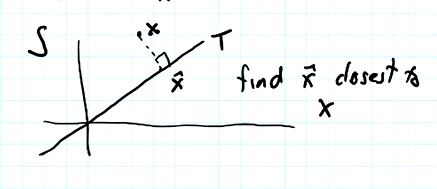
\includegraphics[width=0.5\linewidth]{6250-L9-IMG1.JPG}
 \end{figure}
\underline{Proof} \\
Start with 2.: \\
Let $\hat{\mathbf{x}}$ be the vector that satisfies $\hat{\mathbf{e}} = \mathbf{x} - \hat{\mathbf{x}} \perp T$ \\
Let $\mathbf{y}$ be any other vector in T, $\mathbf{e} := \mathbf{x} - \mathbf{y}$ \\
We will show that $||\mathbf{e}|| > ||\hat{\mathbf{e}}||$ \\
\begin{equation*}
    ||\mathbf{e}||  = ||\mathbf{x} - \mathbf{y}||^2 = ||\mathbf{x} - \mathbf{y} + \hat{\mathbf{x}} - \hat{\mathbf{x}}||^2  = ||\mathbf{x} - \mathbf{y} + \hat{\mathbf{x}} + \hat{\mathbf{e}} - \mathbf{x}||^2 = ||\hat{\mathbf{e}} - \mathbf{y} + \hat{\mathbf{x}}||^2 = ||\hat{\mathbf{e}} - (\mathbf{y} - \hat{\mathbf{x}})||^2
\end{equation*}
\begin{equation*}
    = \langle \hat{\mathbf{e}} - (\mathbf{y} - \hat{\mathbf{x}}), \hat{\mathbf{e}} - (\mathbf{y} - \hat{\mathbf{x}}) \rangle
\end{equation*}
\begin{equation*}
    = ||\hat{\mathbf{e}}||^2 + \underbrace{||\mathbf{y} - \hat{\mathbf{x}}||^2}_{\text{not zero}} - \cancelto{0}{\langle \hat{\mathbf{e}}, \mathbf{y}-\hat{\mathbf{x}}\rangle} - \cancelto{0}{\langle \mathbf{y}-\hat{\mathbf{x}}, \hat{\mathbf{e}}\rangle}
\end{equation*}
$\therefore ||\mathbf{e}|| > ||\hat{\mathbf{e}}||.$
Geometrically: \\
\begin{figure}[H]
    \centering
    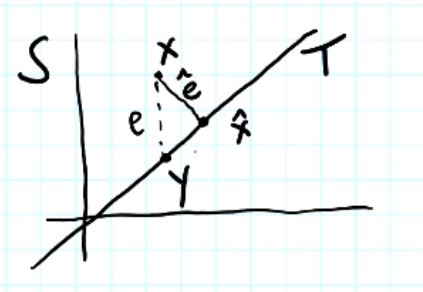
\includegraphics[width=0.5\linewidth]{6250-L9-IMG2.JPG}
\end{figure}

\newpage
\lecture{Approximations in Hilbert Spaces pt 2}
\color{ForestGreen}
\large{\textbf{Best Approximation}}
\color{Black}\\
We proved there is a unique minimizer (clause 2 from the theorem) in the previous lecture. Now we will prove the first clause. \\
We compute $\hat{\mathbf{x}}$, the optimal point. \\
Let N be the dimension of the subspace T, and let $\mathbf{v}_1,...,\mathbf{v}_n$ be a basis for T. We want to find the set of coefficients $a_1,...,a_n \in \mathbb{C}$ such that 
\begin{equation*}
    \hat{\mathbf{x}}= a_1 \mathbf{v}_1 + a_2 \mathbf{v}_2 + ... + a_N \mathbf{v}_N
\end{equation*}
From the orthogonality principle:
\begin{equation*}
    \langle \mathbf{x} - \hat{\mathbf{x}}, \mathbf{v}_n \rangle = 0 \quad \text{for} \: n=1,...,N
\end{equation*}
so
\begin{equation*}
    \langle \underbrace{\mathbf{x} - \sum_{k=1}^N a_k \mathbf{v}_k}_{\hat{\mathbf{x}}}, \mathbf{v}_n \rangle = 0 \quad \text{for} \: n=1,...,N
\end{equation*}
then
\begin{equation*}
    \langle \mathbf{x},\mathbf{v}_n \rangle = \sum_{k=1}^N a_k  \langle \mathbf{v}_k,\mathbf{v}_n \rangle \quad \text{for} \: n=1,...,N
\end{equation*}
which gives us n linear equations. 
\begin{equation*}
    \underbrace{
        \begin{bmatrix}
            \langle \mathbf{v}_1,\mathbf{v}_1 \rangle & \langle \mathbf{v}_2,\mathbf{v}_1 \rangle & \cdots & \langle \mathbf{v}_N,\mathbf{v}_1 \rangle \\
            \langle \mathbf{v}_1,\mathbf{v}_2 \rangle & \langle \mathbf{v}_2,\mathbf{v}_2 \rangle & \cdots & \langle \mathbf{v}_N,\mathbf{v}_2 \rangle \\
            \vdots & \vdots & \ddots & \vdots \\
            \langle \mathbf{v}_1,\mathbf{v}_N \rangle & \langle \mathbf{v}_2,\mathbf{v}_N \rangle & \cdots & \langle \mathbf{v}_N,\mathbf{v}_N \rangle \\
        \end{bmatrix}    
    }_{\text{\textbf{G}}}
    \underbrace{
        \begin{bmatrix}
            a_1 \\ 
            a_2 \\ 
            \vdots \\
            a_N
        \end{bmatrix}
    }_{\text{\textbf{a}}}
    = 
    \underbrace{
        \begin{bmatrix}
            \langle \mathbf{x},\mathbf{v}_1 \rangle  \\ 
            \langle \mathbf{x},\mathbf{v}_2 \rangle  \\ 
            \vdots \\
            \langle \mathbf{x},\mathbf{v}_N \rangle 
        \end{bmatrix}
    }_{\text{\textbf{b}}}
\end{equation*}
Where \textbf{G} is the Gram matrix or Grammian of the basis ${\mathbf{v}_n}$.
\begin{equation*}
    \mathbf{G} \mathbf{a} = \mathbf{b} \Rightarrow \mathbf{a} = \mathbf{G}^{-1} \mathbf{b}
\end{equation*}
\begin{itemize}
    \item G is invertible because ${\mathbf{v}_n}$ are linearly independent \\
    \item G is conjugate symmetric (Hermitian) i.e. $G = G^H$ \\
\end{itemize}
There is a unique a therefore, only on $\hat{\mathbf{x}}$ that satisfies $\mathbf{x} - \hat{\mathbf{x}} \perp T$

\newpage
\lecture{Approximation Example}
\color{ForestGreen}
\large{\textbf{Approximation Example}}
\color{Black}\\
Let S = $\mathbb{R}^3$, with standard inner product $\langle \mathbf{x},\mathbf{y} \rangle = \sum_{n=1}^3 x_n y_n$ and the induced norm $||\cdot||_2$
\begin{equation*}
    T = \text{Span}\left(
    \begin{bmatrix}
        1 \\
        1 \\
        1 \\
    \end{bmatrix},
    \begin{bmatrix}
        1 \\
        -1 \\
        1 \\
    \end{bmatrix}
    \right), \quad
    \mathbf{x} = \begin{bmatrix}
        -2 \\
        1 \\
        3 \\
    \end{bmatrix}
\end{equation*}
Find $\hat{\mathbf{x}} \in T $  that is closest to $\mathbf{x}$.\\ \\
We start by building the Gram matrix: 
\begin{equation*}
    \mathbf{G} = 
    \begin{bmatrix}
        \langle \mathbf{v}_1,\mathbf{v}_1 \rangle & \langle \mathbf{v}_2,\mathbf{v}_1 \rangle & \cdots & \langle \mathbf{v}_N,\mathbf{v}_1 \rangle \\
        \langle \mathbf{v}_1,\mathbf{v}_2 \rangle & \langle \mathbf{v}_2,\mathbf{v}_2 \rangle & \cdots & \langle \mathbf{v}_N,\mathbf{v}_2 \rangle \\
        \vdots & \vdots & \ddots & \vdots \\
        \langle \mathbf{v}_1,\mathbf{v}_N \rangle & \langle \mathbf{v}_2,\mathbf{v}_N \rangle & \cdots & \langle \mathbf{v}_N,\mathbf{v}_N \rangle \\
    \end{bmatrix}   
    = 
    \begin{bmatrix}
        \langle \mathbf{v}_1,\mathbf{v}_1 \rangle & \langle \mathbf{v}_2,\mathbf{v}_1 \rangle  \\
        \langle \mathbf{v}_1,\mathbf{v}_2 \rangle & \langle \mathbf{v}_2,\mathbf{v}_2 \rangle \\
    \end{bmatrix}   
    =
    \begin{bmatrix}
        3 & 1  \\
        1 & 3 \\
    \end{bmatrix}  
\end{equation*}
\begin{equation*}
    \mathbf{b} = 
    \begin{bmatrix}
        \langle \mathbf{x},\mathbf{v}_1 \rangle  \\ 
        \langle \mathbf{x},\mathbf{v}_2 \rangle  \\ 
        \vdots \\
        \langle \mathbf{x},\mathbf{v}_N \rangle 
    \end{bmatrix}
    =
    \begin{bmatrix}
        \langle \mathbf{x},\mathbf{v}_1 \rangle  \\ 
        \langle \mathbf{x},\mathbf{v}_2 \rangle  \\  
    \end{bmatrix}
    =
    \begin{bmatrix}
        2 \\
        0 \\
    \end{bmatrix}
\end{equation*}
\begin{equation*}
    \mathbf{a} = \mathbf{G}^{-1} b
\end{equation*}
Refresher: The inverse of a 2x2 matrix is 
\begin{equation*}
    \begin{bmatrix}
        a & b \\
        c & d \\
    \end{bmatrix}^{-1}
    = \frac{1}{ad-bc} 
    \begin{bmatrix}
        d & -b \\
        -c & a \\
    \end{bmatrix}
\end{equation*}
Here
\begin{equation*}
    \mathbf{G}^{-1}
    = \frac{1}{8} 
    \begin{bmatrix}
        3 & -1 \\
        -1 & 3 \\
    \end{bmatrix}
\end{equation*}
\begin{equation*}
    \mathbf{G}^{-1} \mathbf{b}
    = \frac{1}{8} 
    \begin{bmatrix}
        3 & -1 \\
        -1 & 3 \\
    \end{bmatrix}
    \begin{bmatrix}
        2 \\
        0 \\
    \end{bmatrix}
    =
    \frac{1}{4} 
    \begin{bmatrix}
        3 \\
        -1 \\
    \end{bmatrix}
\end{equation*}
\begin{equation*}
    \hat{\mathbf{x}} = \frac{3}{4} 
    \begin{bmatrix}
        1 \\
        1 \\
        1 \\
    \end{bmatrix}
    - \frac{1}{4}
    \begin{bmatrix}
        1 \\
        -1 \\
        1 \\
    \end{bmatrix}
    =
    \begin{bmatrix}
        \frac{1}{2} \\
        1 \\
        \frac{1}{2} \\
    \end{bmatrix}
\end{equation*}
$\hat{\mathbf{x}} $ is our solution to find the best approximation in the subspace. \\
We can double check:
\begin{equation*}
    \mathbf{x} - \hat{\mathbf{x}} = 
    \begin{bmatrix}
        -2.5 \\
        0 \\
        2.5 \\
    \end{bmatrix}
\end{equation*}
\begin{equation*}
    \langle \mathbf{x} - \hat{\mathbf{x}}, \hat{\mathbf{x}} \rangle = 
    \begin{bmatrix}
        -2.5 &
        0 &
        2.5 \\
    \end{bmatrix} \cdot
    \begin{bmatrix}
        \frac{1}{2} \\
        1 \\
        \frac{1}{2} \\
    \end{bmatrix} = 
    0. 
\end{equation*}

\newpage
\lecture{Orthobases}
\color{ForestGreen}
\large{\textbf{Orthogonal Bases}}
\color{Black}\\
A collection of vectors $\{ \mathbf{v}_1, ..., \mathbf{v}_n \}$ in a finite-dimensional vector space S is called an \underline{orthogonal basis} if 
\begin{enumerate}
    \item span($\{ \mathbf{v}_1, ..., \mathbf{v}_n \}$) = S 
    \item $\mathbf{v}_j \perp \mathbf{v}_k$ (i.e. $\langle \mathbf{v}_j, \mathbf{v}_k \rangle = 0 $ for all $j \neq k$
\end{enumerate}
in addition, if the vectors are normalized 
\begin{equation*}
    ||\mathbf{v}_n|| = 1 \text{ for } n=1,...,N
\end{equation*}
we have an \underline{orthonormal} basis or \underline{orthobasis}. \\ 
\underline{Examples} \\
1. S = $\mathbb{R}^2$ with standard inner product 
\begin{equation*}
    \mathbf{v}_1 = \frac{1}{\sqrt2} 
    \begin{bmatrix}         
        1 \\         
        1 \\         
    \end{bmatrix} \quad          
    \mathbf{v}_2 = \frac{1}{\sqrt2} 
    \begin{bmatrix} 
        1 \\    
        -1 \\ 
    \end{bmatrix} 
\end{equation*}
the $\frac{1}{\sqrt2}$ normalizes the vectors. \\
Alternative example: 
\begin{equation*}
    \mathbf{v}_1 = 
    \begin{bmatrix}
        1 \\
        0 \\
    \end{bmatrix}
    \quad 
    \mathbf{v}_2 = 
    \begin{bmatrix}
        0 \\
        1 \\
    \end{bmatrix}    
\end{equation*}
2. S = space of piecewise constant functions on $[0, 1/4), [1/4, 1/2), [1/2, 3/4), [3/4, 1]$.
We define the inner product as 
\begin{equation*}
    \langle \cdot , \cdot \rangle = \int_0^1 \mathbf{v}_i(t) \mathbf{v}_j (t) dt
\end{equation*}
\begin{figure}[H]
    \centering
    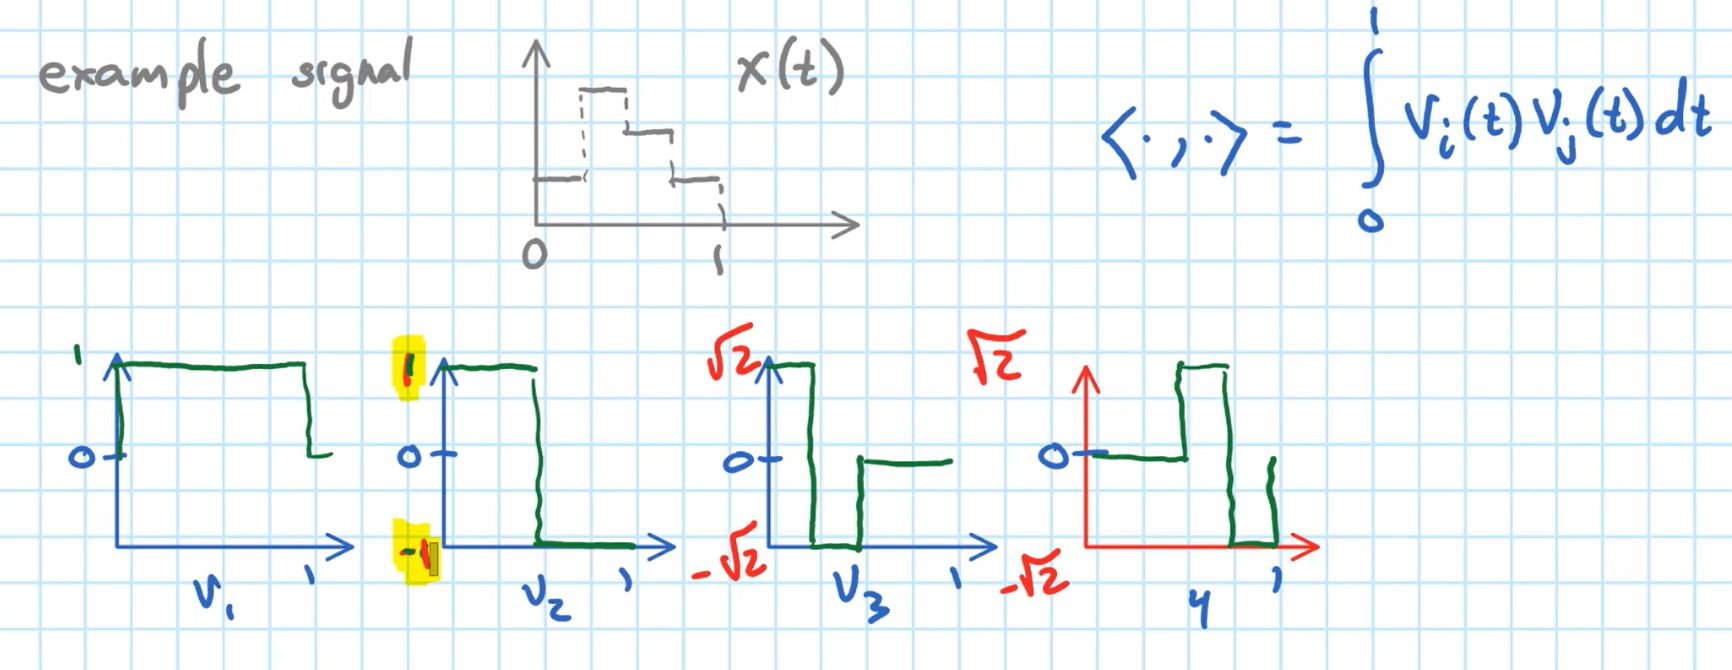
\includegraphics[width=0.75\linewidth]{6250-L12-IMG1.JPG}
\end{figure}
One way to construct a basis for the example signal in grey is to just use one basis signal for every level $x(t)$. An alternative is to use the basis functions at the bottom of the image. \\
3. $\{ \mathbf{v}_k(t) = \frac{1}{\sqrt{2 \pi}}e^{jkt}, k \in \mathbb{Z}\}$ is an orthobasis for $L_2([0, 2\pi])$ \\
(standard inner product) \\
\begin{equation*}
    \langle \mathbf{v}_k(t), \mathbf{v}_{\ell}(t) \rangle = \frac{1}{2\pi} \int_0^{2\pi} e^{jt(k-\ell)} dt = 
    \begin{cases}
        1 & k=\ell \\
        0 & k \neq \ell
    \end{cases}   
\end{equation*}
When $k \neq \ell$, we integrate over the entire period of a sinusoid, which cancels out to zero. \\
4. $B_{\frac{\pi}{T}} (\mathbb{R}) = $ real-valued functions which are bandlimited to $\frac{\pi}{T}$ (standard inner product)
The set of functions
\begin{equation*}
    \left\{v_n(t) = \sqrt T \frac{sin(\pi (t-nT)/T)}{\pi (t-nT)} , n \in \mathbb{Z} \right\}
\end{equation*}
is an orthobasis for $B_{\frac{\pi}{T}}$ \\
This says that 
\begin{equation*}
    \boxed{x(t) = \sum_n \underbrace{x[n]}_{a_n} \sqrt T \frac{sin(\pi(t-nT)/T}{\pi (t-nT)}}
\end{equation*}
(reconstruction of a signal from samples) \\

\newpage
\lecture{Orthobasis Expansions}
\color{ForestGreen}
\large{\textbf{Linear Approximation with Orthobases}}
\color{Black}\\
To approximate $ \mathbf{x} \in S$ with $\hat{\mathbf{x}} \in T$ where S is a Hilbert space with subspace T: \\
if $\{ \mathbf{v}_1,...,\mathbf{v}_n \}$ is a basis for T then $\hat{\mathbf{x}} = a_1 \mathbf{v}_1 + ... + a_n \mathbf{v}_n$ and $\mathbf{a} = G^{-1} \mathbf{b} $ as defined in lecture 10. \\
If $\{ \mathbf{v}_1,...,\mathbf{v}_n \}$ is orthonormal then $G = I$ 
\begin{equation*}
    \underbrace{
        \begin{bmatrix}
            a_1 \\ 
            a_2 \\ 
            \vdots \\
            a_N
        \end{bmatrix}
    }_{\text{\textbf{a}}}
    = 
    \underbrace{
        \begin{bmatrix}
            \langle \mathbf{x},\mathbf{v}_1 \rangle  \\ 
            \langle \mathbf{x},\mathbf{v}_2 \rangle  \\ 
            \vdots \\
            \langle \mathbf{x},\mathbf{v}_N \rangle 
        \end{bmatrix}
    }_{\text{\textbf{b}}}
    \quad \text{i.e. } \: a_i = \langle \mathbf{x}, \mathbf{v}_i \rangle \quad \text{\underline{\textcolor{red}{Only for an orthobasis!}}}
\end{equation*}
\begin{equation*}
    \hat{\mathbf{x}} = \sum_{k=1}^n \langle \mathbf{x}, \mathbf{v}_k \rangle \mathbf{v}_k
\end{equation*}
\color{ForestGreen}
\large{\textbf{Orthobasis expansion}}
\color{Black}\\
If T is the whole space S, given $ \mathbf{x} \in S$, the closest point in T is the point itself. 
\begin{equation*}
    \mathbf{x} = \sum_{n=1}^N \langle \mathbf{x}, \mathbf{v}_n \rangle \mathbf{v}_n \quad \text{ for all } \mathbf{x} \in S
\end{equation*}
also works for infinite-dimensional spaces as long as 
\begin{equation*}
    \sum_{n=-\infty}^{\infty} |\langle \mathbf{x}, \mathbf{v}_n|^2 < \infty \Rightarrow \mathbf{x} = \sum_{n=-\infty}^\infty \langle \mathbf{x}, \mathbf{v}_n \rangle \mathbf{v}_n
\end{equation*}

\newpage
\lecture{Parseval's Theorem++}
Let S be a Hilbert space with an inner product $\langle \cdot, \cdot \rangle_S$ which induces a norm $||\cdot||_S$. Let $\{\mathbf{v}_k\}_k$ be an orthobasis for S. \\
Then for every $\mathbf{x}, \mathbf{y} \in S$,
\begin{equation*}
    \langle \mathbf{x}, \mathbf{y} \rangle_S = \sum_k \alpha_k \bar \beta_k = \langle \boldsymbol{\alpha}, \boldsymbol{\beta} \rangle_{\ell_2}
\end{equation*}
Where $\alpha_k = \langle \mathbf{x}, \mathbf{v}_k \rangle_S $ and $\beta_k = \langle \mathbf{y}, \mathbf{v}_k \rangle _S$. We call them the transform coefficients. The significance of this is that 
\begin{equation*}
    \langle \mathbf{x}, \mathbf{y} \rangle_S = \langle \boldsymbol{\alpha}, \boldsymbol{\beta} \rangle_{\ell_2}
\end{equation*}
\underline{An orthobasis can make every Hilbert space equivalent to $\ell_2$.} With Parseval's theorem, we are used to seeing: 
\begin{equation*}
    ||\mathbf{x}||_S^2 = ||\boldsymbol{\alpha}||_2^2
\end{equation*}
Proof sketch:
\begin{equation*}
    \mathbf{x} = \sum_k \alpha_k \mathbf{v}_k \quad \mathbf{y} = \sum_k \beta_k \mathbf{v}_k
\end{equation*}
\begin{equation*}
    \langle \mathbf{x}, \mathbf{y} \rangle_S = \langle \sum_k \alpha_k \mathbf{v}_k, \sum_{\ell} \beta_{\ell} \mathbf{v}_{\ell} \rangle = \sum_k \alpha_k \langle \mathbf{v}_k, \sum_{\ell} \beta_{\ell} \mathbf{v}_{\ell} \rangle
\end{equation*}
\begin{equation*}
    = \sum_k \alpha_k \sum_{\ell} \beta_{\ell} \underbrace{\langle \mathbf{v}_k, \mathbf{v}_{\ell} \rangle}_{a}
\end{equation*}
Where the inner product denoted by a $=0 \text{ for } k \neq \ell \text{ and } = 1\text{ for } k \neq \ell$
\begin{equation*}
   \boxed{ \langle \mathbf{x}, \mathbf{y} \rangle_S = \sum_k \alpha_k \bar \beta_k}
\end{equation*}

% Week 4 lectures
\section*{Week 4}
\addcontentsline{toc}{section}{Week 4}
\markboth{Week 4}{}









\end{document}

